%***************************************PREAMBLE***************************************
\documentclass[a4paper,12pt]{article}

\usepackage[utf8]{inputenc}
\usepackage[margin=0.7in]{geometry}
\usepackage[T1]{fontenc}
\usepackage{graphicx}
\usepackage{float}
\usepackage{setspace}
\usepackage{appendix}
\usepackage{amsmath}
\usepackage{cite}
\usepackage{caption}
\usepackage{subcaption}


%***************************************DOCUMENT***************************************

\DeclareMathOperator*{\argmin}{\arg\!\min}
\DeclareMathOperator*{\argmax}{\arg\!\max}

\setlength{\parindent}{0em}

\begin{document}
	\fontfamily{ptm}\selectfont
	%%%%%%%%%%%%%%%%%%%%%%%%%%%%%%%%%%%%%%%COVERSHEET%%%%%%%%%%%%%%%%%%%%%%%%%%%%%%%%%%%%%%%
	\begin{titlepage}
		\setlength{\voffset}{-0.8in}
		\noindent \makebox[\textwidth]{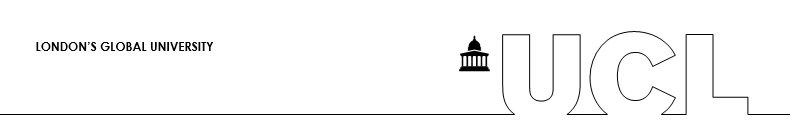
\includegraphics[width=1.2\textwidth]{images/Coversheet_Header.png}}
	
			\vspace{15mm}
			
			\begin{center}
				{\Huge \textbf{COMP0037 \\ \vspace{10mm} Report}}
			
				\vspace{8mm}
			
				\begin{spacing}{1.8}
					{\huge Exploration in Unknown Environments}
				\end{spacing}
		
			
				\vspace{12mm}
			
				{\LARGE \textbf{Group AS}}
				
				\vspace{10mm}
				
				\begin{tabular}{ll}
					\underline{\textbf{Student Name}}  & \hspace{4mm} \underline{\textbf{Student number}} \vspace{2mm} \\
					Arundathi Shaji Shanthini & \hspace{4mm} 16018351 \\ 
					Dmitry Leyko & \hspace{4mm}  16021440\\ 
					Tharmetharan Balendran & \hspace{4mm} 17011729\\ 
				\end{tabular}
				
				\vspace{13mm}
				
				\begin{tabular}{ll}
					\textbf{Department:} &  Department of Electronic and Electrical Engineering\\ \vspace{3mm}
					\textbf{Submission Date:} &  31\textsuperscript{st} of March 2020
				\end{tabular}
			\end{center}
	\end{titlepage}
	%%%%%%%%%%%%%%%%%%%%%%%%%%%%%%%%%%%%%%
	
	\pagebreak
	
	\tableofcontents
	
	\pagebreak
	
	%%%%%%%%%%% PART 1 %%%%%%%%%%%%%%%%%
	\section{Reactive Planner}
		\begin{figure}[H]
			\centering
			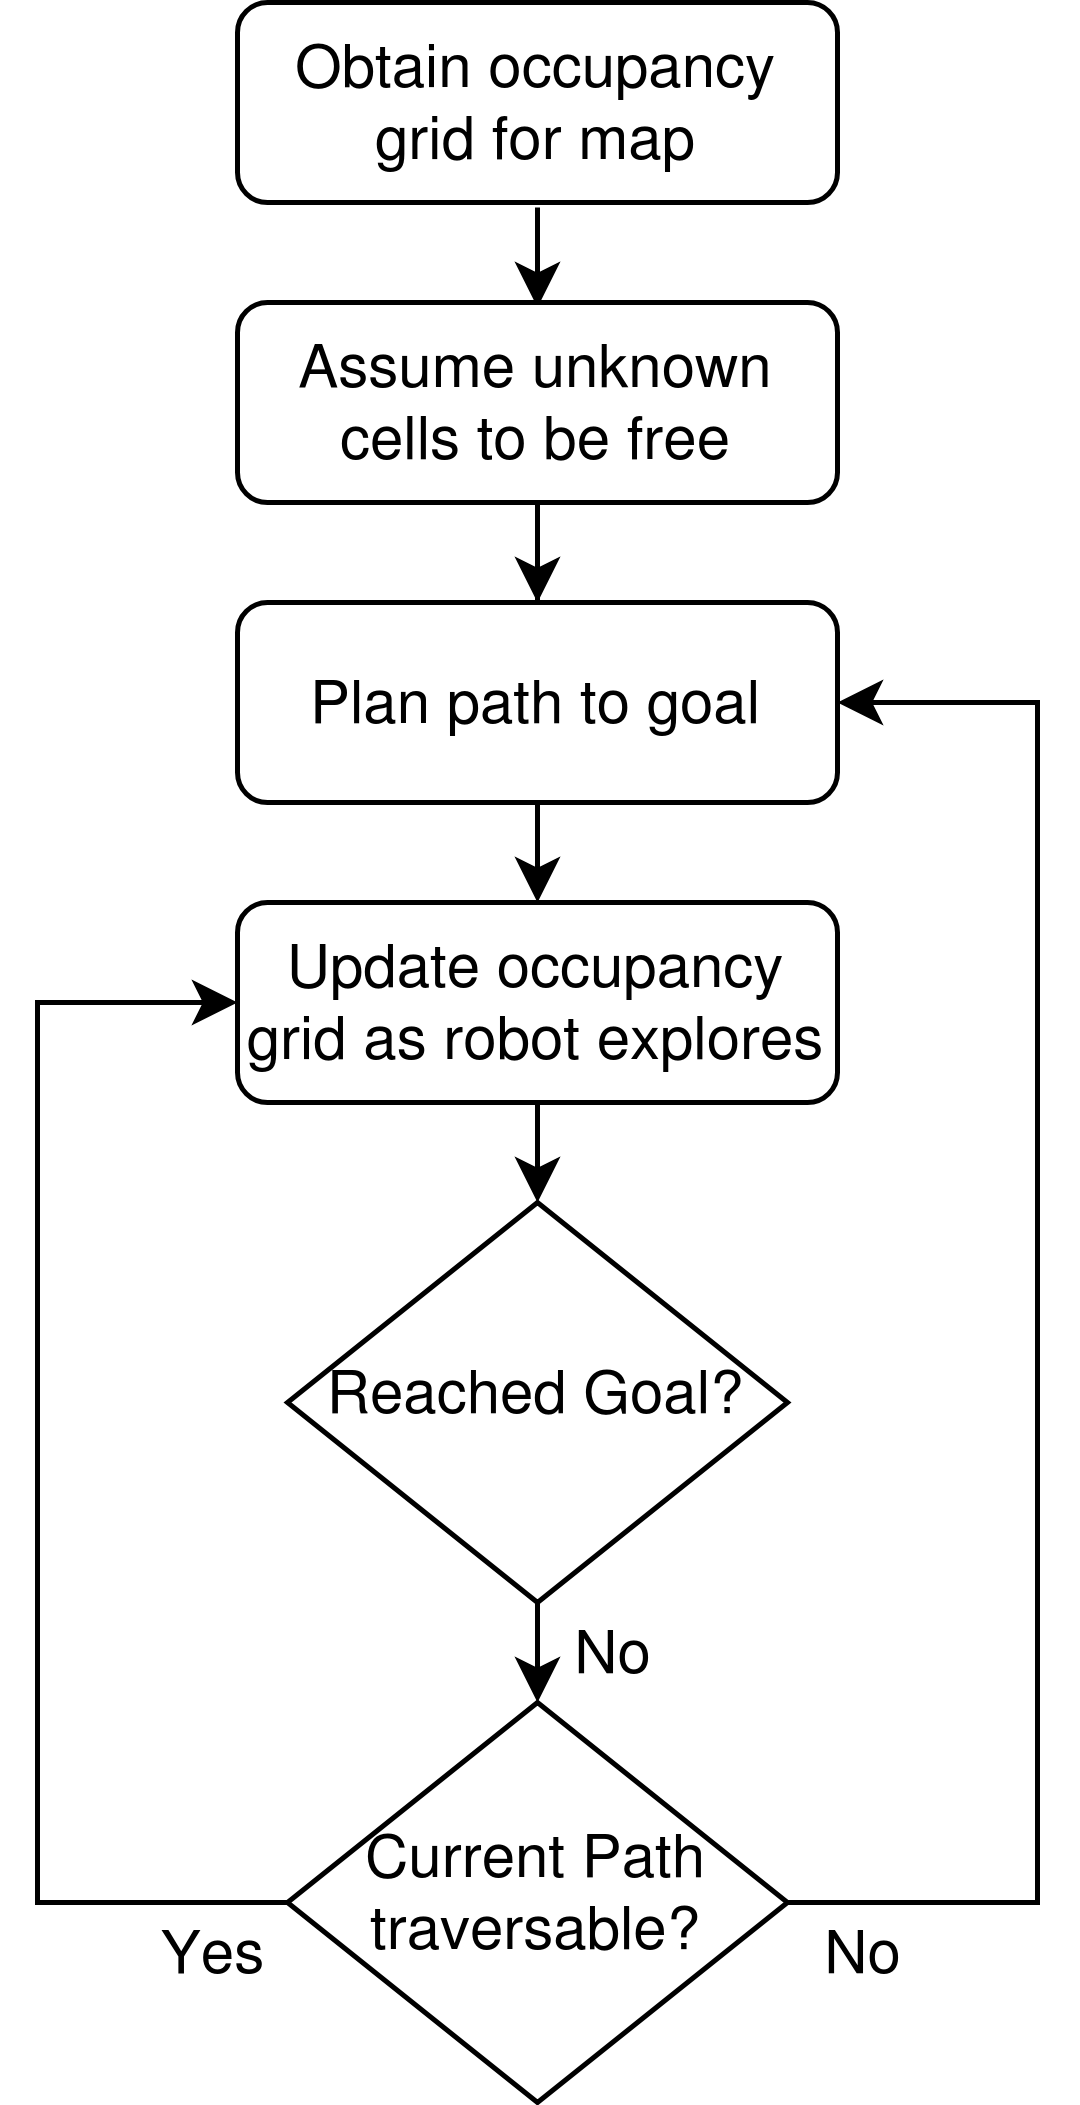
\includegraphics[scale=0.13]{images/reactivePlannerFlowchart.png}
			\caption{Flowchart for the reactive planner}
			\label{reactivePlannerFlowchart}
		\end{figure}
	
		\subsection{Our Implementation of a Reactive Planner}

			A reactive planner is able to adapt its path based on the information it obtains about the environment as it explores it. The high-level functionality of a general reactive planner is described in the flowchart in Fig.\ref{reactivePlannerFlowchart}. The reactive planner initially utilizes the available occupancy grid and computes a search grid from this grid assuming any unknown cells to be free. The computation of the search grid instead of utilizing the occupancy grid directly will prevent the robot from ending up too close to the walls. The planner then plans a path using this assumption and starts to traverse the path. The robot will explore the environment as it traverses the path and if new information suggests that the currently planned path is no longer traversable, a new path is planned using the new occupancy grid and search grid. This process is repeated until the robot arrives at the goal.
			\\
			\\
			As a means of testing the code the robot was set to visit a list of goals on the factory map. The final mapper node occupancy grid is shown in Fig.\ref{mapperNodeOccupancyGrid}. It is clear to see that there are inaccuracies in the mapping of the world as well as some areas which have still not been explored completely. The inaccuracies occur as a result of rounding errors and other noise due to timing mismatch (caused by networking delays), these errors are mostly corrected as the robot re-explores an area.
			\\
			\\
			The way the map is updated is using the laser range finder that the robot is equipped with. Depending on the reflections of this laser, the environment surrounding the robot can be mapped. Fig.\ref{robotLaserRange} depicts an instance in time of the robot. The red lines represent the individual laser beams used to map the surrounding environment. It is clear to see that the laser beam is stopped (and reflected) by the opaque walls. By measuring the time taken for the reflected beam to return, the distance to the opaque object can be calculated. In addition to this, it can also be seen that some of the beams stop despite not having hit any opaque objects. This is due to the maximum measurable range of the laser range detector. 

			\begin{figure}[H]
				\centering
				\begin{subfigure}{.5\textwidth}
					\centering
					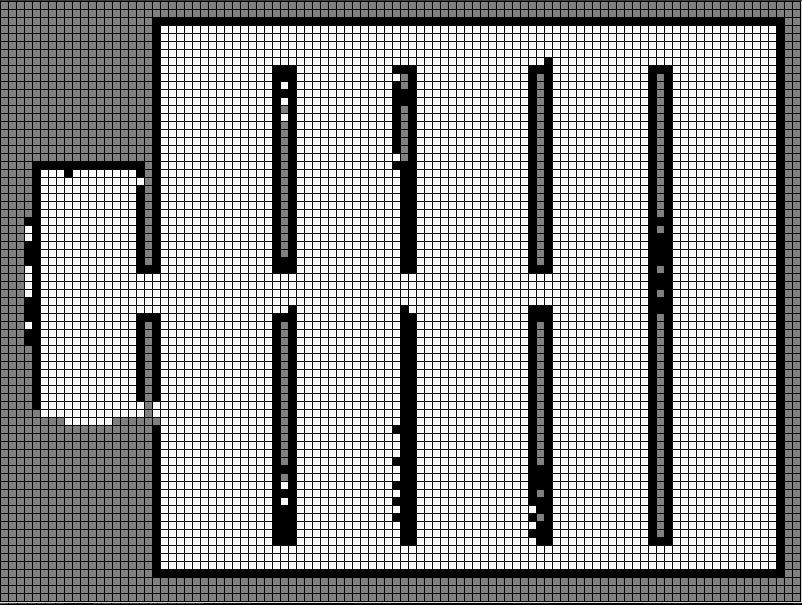
\includegraphics[width=.7\linewidth]{images/mapperNodeOccupancyGrid.png}
					\caption{Mapper Node occupancy grid}
					\label{mapperNodeOccupancyGrid}
				\end{subfigure}
				\begin{subfigure}{.5\textwidth}
					\centering
					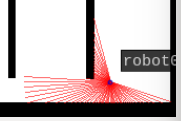
\includegraphics[width=.7\linewidth]{images/robotLaserRange.png}
					\caption{Robot Laser Range Finder}
					\label{robotLaserRange}
				\end{subfigure}
				\caption{a) Mapper occupancy grid at the end of traversing the set of goals. b) The robot traversing the map with the laser range finder visualized by the red lines. The maximum range as well as the opaque walls preventing the laser from passing through can also be seen.}
				\label{ReactivePlannerFigs}
			\end{figure}

		\subsection{Improving the performance of the Reactive Planner}

			Our implementation of a reactive planner is quite inefficient and may be computationally intense. The current global planner that is used to plan the paths uses an implementation of Dijkstra's algorithm to plan the path. One way of improving the performance is by utilizing the A* algorithm. This way fewer cells will be considered when planning the path resulting in a lower computational cost.
			\\
			\\
			Another method of improving efficiency is to prevent the algorithm from having to re-plan the whole path. In a dynamic environment, obstacles may move in and out of the robot's path. Therefore, sometimes it may be sufficient to take a remedial action to overcome/avoid the obstacle. This may involve simply waiting for the obstacle to pass or in more complicated cases it may involve the robot moving the obstacle out of the way. However, not all obstacles may be overcome in such a way. For example, a newly discovered wall will neither move on its own nor is it possible for the robot to move the wall. In such a case, a local planner may be utilized to plan a path around the obstacle. This involves planning a path to another point on the proposed path and thereby avoiding the obstacle. These local planners are very responsive and generally utilize gradient-based techniques which use physics-based approximations. Despite being fast and responsive, they generally get stuck in local minima. 
			
	%%%%%%%%%%%%%%%%%%%%%%%%%%%%%%%%%%%%%%
	
	%%%%%%%%%%% PART 2 %%%%%%%%%%%%%%%%%
	\section{Frontier-Based Exploration System}

		\subsection{Frontier Exploration}

			A frontier is a region or group of cells which marks the boundary between the known open space of the environment and the unknown and unexplored space of the environment. For a cell to be classified as a frontier cell, it's state must be known to be free and it must have an adjacent cell of which the state is not known. Two adjacent frontier cells are considered to be part of the same frontier (i.e. the same boundary) if the previous cell scanned was also a frontier cell.\cite{keidar2011fast}
			
			An example of a frontier can be found in Fig \ref{frontierExample}. Frontiers are useful in exploring unknown environments as travelling to these cells will allow the robot to find out more about the unknown portion of the map. There are multiple algorithms for detecting frontiers and choosing the optimal next destination to allow the robot to maximise it's knowledge of the surrounding. Some of these approaches will be discussed in this chapter.

			\begin{figure}[H]
				\centering
				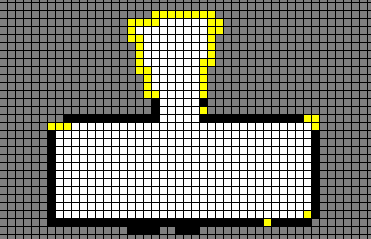
\includegraphics[scale=0.6]{images/frontierExample.png}
				\caption{A portion of a partially explored map. Cells marked white are known to be free while cells marked black are known to occupied while cells marked grey are unknown. The cells marked yellow are known to be free and have neighbouring unknown cells (i.e. they are frontier cells).}
				\label{frontierExample}
			\end{figure}

			\subsection{Frontier Detection}

				Two algorithms for frontier detection will be discussed. One of them is Wave-front Frontier Detection (WFD) and the other is Fast Frontier Detection (FFD). As the name implies the FFD algorithm is less computationally intense and scales better to larger problems due to its higher efficiency. However, both of these algorithm provide the same result in identifying frontiers.
				
				\subsubsection{Wave-front Frontier Detection}

				The WFD algorithm works by implementing two nested Breadth First Search (BFS) algorithms. This search algorithm utilizes a First In First Out (FIFO) queue to manage the cells that are searched over. The starting cell is set as the current pose of the robot. From this cell, the outer BFS algorithm traverses neighbouring cells and checks if each one of them is a frontier cell. If a frontier cell is found the cell is added to the FIFO queue of the inner BFS algorithm and the neighbouring cells of this cell are checked to see if they too are frontier cells. If they are then they are added to the inner queue and this continues until all frontier cells in the cluster are found. Once no more cells are on the queue, we break out of the inner BFS and continue on the outer BFS until another frontier cell is encountered. The pseudocode for this algorithm can be found in Fig. \ref{wfdPseudocode}. In this pseudocode the cells are assigned to 5 different states: \textbf{Unvisited}, \textbf{Map-Open List}, \textbf{Map-Close List}, \textbf{Frontier-Open List} and \textbf{Frontier-Close List}. Initially all cells are unvisited. If enqueued by the outer BFS, the cell is labelled as \textit{'Map-Open List'} and once dequeued by the outer BFS it is labelled as \textit{'Map-Close List'}. Similarly if enqueued by the inner BFS, the cell is labelled as \textit{'Frontier-Open List'} and once dequeue it is labelled as \textit{'Frontier-Close List'}. 
				
				\subsubsection{Fast Frontier Detection}

				The FFD algorithm is an extension to the WFD algorithm. The WFD algorithm on its own identifies frontiers over the whole map every time the map is updated. This means that frontiers that have already been identified that didn't change will still have to re-identified by the algorithm. FFD overcomes this inefficiency by computing the frontiers of only the cells identified by the robot's laser readings. By doing so, the number of cells that are traversed in the search is greatly reduced, especially if the environment is of a greater size than considered in this coursework (e.g. 3D with environment broken discretized using a higher resolution). Once the algorithm has computed the frontiers of the cells identified by the laser scan, the old frontiers and the new frontiers from the laser scan are compared. The pseudocode for this algorithm is shown in Fig. \ref{ffdPseudocode}. This pseudocode tackles the identification of cells from raw laser readings as well which will not be discussed. The main focus is the section of code labelled "maintenance of previously detected frontiers". This section of the code aims to gain information about the frontiers of the whole map by using the old frontiers on the map and the frontiers of the laser scan. In this step multiple checks are performed: if a newly identifier frontier already exists, to see if an old frontier is no longer a frontier and to see if previously separate frontiers are now joined. 
				
				\begin{figure}[H]
					\centering
					\begin{subfigure}{.5\textwidth}
						\centering
						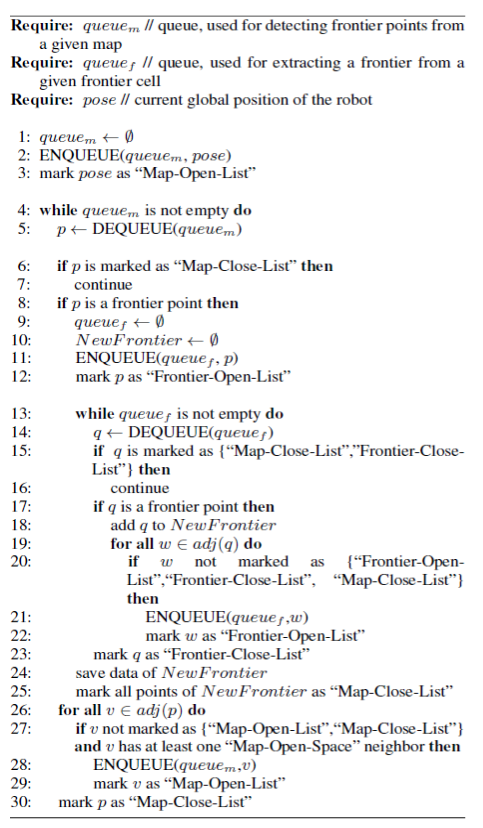
\includegraphics[width=.9\linewidth]{images/wfdPseudocode.png}
						\caption{Wave-front Frontier Detection Pseudocode}
						\label{wfdPseudocode}
					\end{subfigure}%
					\begin{subfigure}{.5\textwidth}
						\centering
						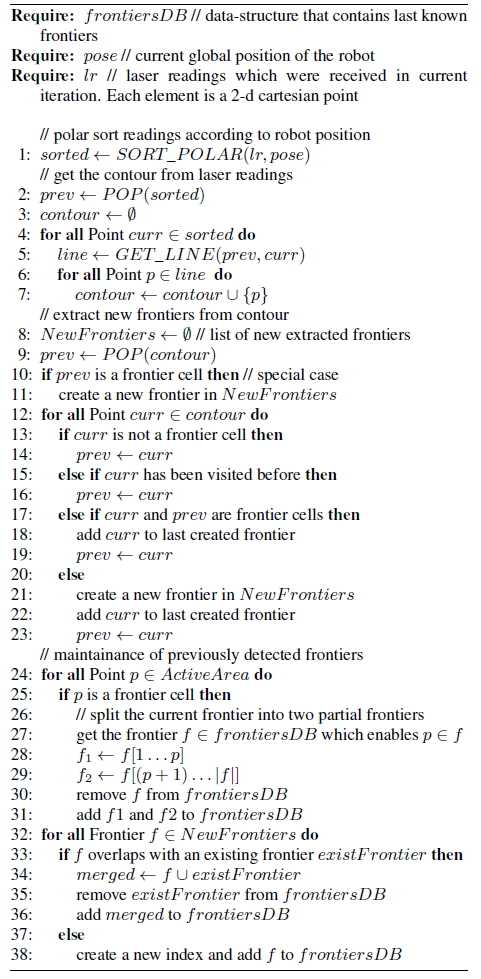
\includegraphics[width=.9\linewidth]{images/ffdPseudocode.png}
						\caption{Fast Frontier Detection Pseudocode}
						\label{ffdPseudocode}
					\end{subfigure}
					\caption{Pseudocode for the two frontier detection algorithms discussed. \cite{topiwala2018frontier, keidar2011fast}}
					\label{frontierSearchPseudocode}
				\end{figure}

			\subsection{Waypoint Selection}

				Once the frontiers are identified the robot needs to decide which point on which frontier it should travel to next. The next destination should be chosen to maximize the amount of new information that can be obtained. For this there are two main methods, heuristic based approach and information based approach. Using these, the robot will be able to pick the next waypoint to move to. 

				\subsubsection{Heuristic Approaches}

					Heuristics can be used to choose the next frontier to travel to. Two main heuristics exist: the largest frontiers and the closest frontier. The largest frontier heuristic chooses the frontier with the largest number of frontier cells as the frontier to travel to next. Which cell of this frontier to travel to may be decided by the closest cell (smallest Euclidean distance to the robot) or the middle cell of the frontier. The idea of choosing the largest frontier as the next frontier is based on the idea that the largest frontier will give the robot the largest field of view to explore the unknown cells. The other heuristic is the distance. In this case the frontier with the smallest Euclidean distance to the robot will be chosen. This approach puts less emphasis on the information gained and aims to improve the time taken to explore the whole map. This is due to the fact that where the size heuristic approach may result in the robot going back and forth between two large frontiers, the distance heuristic approach is likely to result in the robot covering all frontiers as it travels. 

				\subsubsection{Information Based Approach}

					This method aims to compute the uncertainty in the map and choses a point that maximizes the amount of information that can be gained about the surrounding environment. The approach utilizes a probabilistic approach and the concept of entropy. The entropy of a singular cell is computed by the equation given in Eq. \ref{eq:singleCellEntropy}. This approach will be discussed in more detail in later chapters.

					\begin{equation}
						H \left(\textbf{c}\right) = -\left(1-p\left(\textbf{c}\right)\right)ln\left(1-p\left(\textbf{c}\right)\right) - p\left(\textbf{c}\right)ln \; p\left(\textbf{c}\right)
						\label{eq:singleCellEntropy}
					\end{equation}

			\subsection{Reference Exploration Algorithm}

				The algorithm implemented out of the box was purposefully inefficient. To choose a new destination, the algorithm traverses over all the cells and identifies if they are frontier cells or not. The search does not implement a queue but rather starts from the coordinate $(0,0)$ and uses two for loops to iterate over columns and rows. The chosen destination is set to be the frontier closes to the point $(0,\frac{Y}{2})$ where $Y$ is the height of the grid. This uses the assumption that the robot will start off in the central left position (close of the stated coordinate). Therefore, it will initially explore cells that are close to it and slowly work its way to the right. However, due to the fact that this algorithm has no notion of frontier size or current position of the robot, the choice of the next waypoint is suboptimal. The plot in Fig. \ref{Part2} shows how the exploration time and coverage compare to our own implementation of a explorer algorithm. it is clearly visible that the reference algorithm is relatively inefficient. It should be noted that the coverage that is computed can never be 100\% in the given map. This is due to the fact that the robot cannot gain information about the cells that are within walls or outside of its confined range.  
			
			\subsection{Improving the Exploration Algorithm}

				\begin{figure}[H]
					\centering
					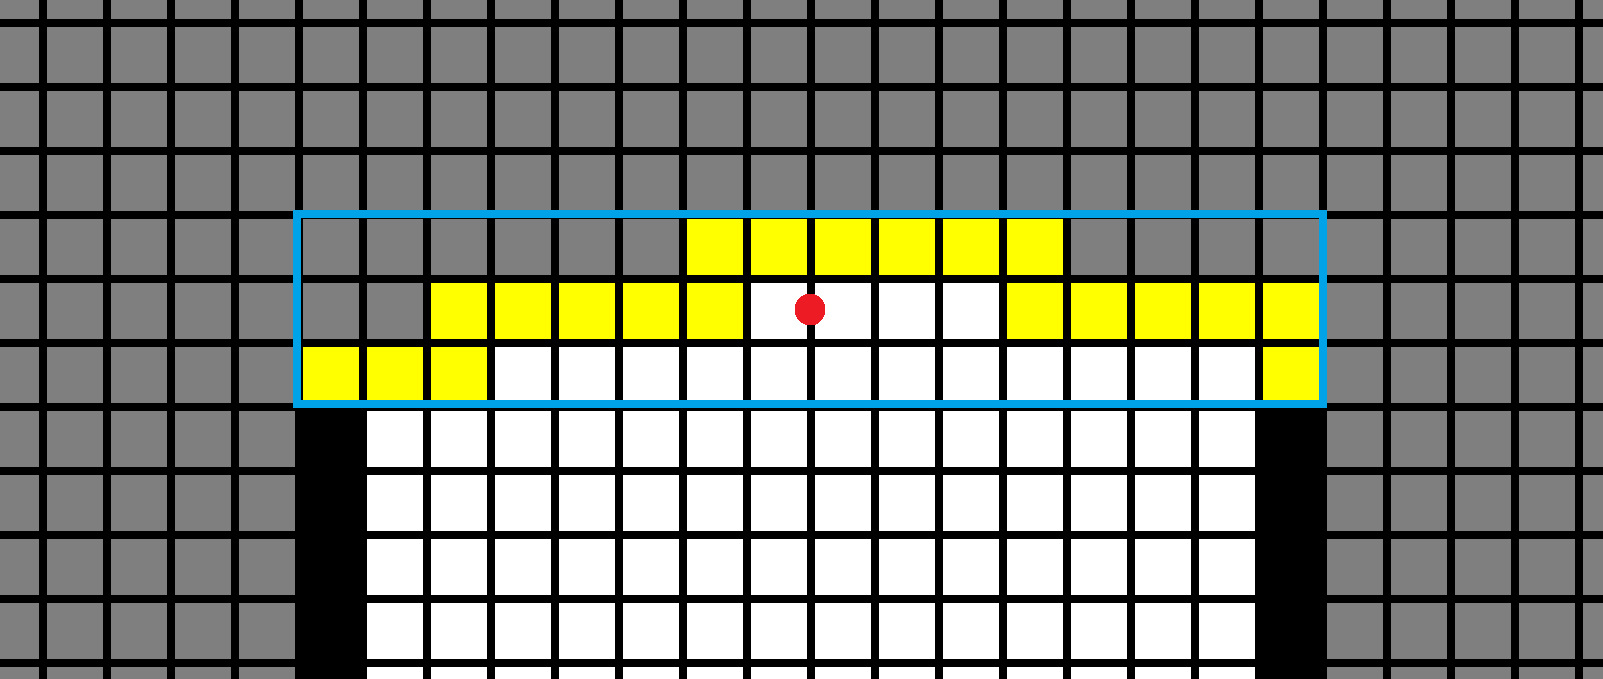
\includegraphics[scale=0.25]{images/middleCellVisualization.png}
					\caption{Visualization of the algorithm that is to compute the middle cell of a frontier. The blue rectangle identifies the extremes of the frontiers and is characterized by the minimum and maximum x and y coordinates of the frontier. The red dot is the middle of the rectangle and the middle cell is chosen as the one that is closest to the red dot.}
					\label{middleCellVisualization}
				\end{figure}

				Our implementation of the exploration algorithm utilizes the WFD algorithm to detect the frontiers of the map. The algorithm has a store of the current frontiers of the map in a priority queue. The priority value is the number of cells in the frontier and the largest frontier is popped first. Every time the map is updated, the WFD algorithm re-identifies the frontiers and updates the list. When a new destination is to be chosen, a frontier is popped from the priority queue and the 2middle" cell is chosen. This notion of "middle" is computed by considering the maximum and minimum x and y coordinates. An illustration of this is shown in Fig. \ref{middleCellVisualization}. The cell closes to the centre of the rectangle outlining the frontiers is chosen. If the algorithm chose a waypoint that was not reached by the robot, this cell is added to a black-list to prevent looping and other bad behaviour. Once black-listed the cell will no longer be chosen as a destination to travel to. The performance of this exploration algorithm is shown in Fig. \ref{Part2} alongside the performance of the baseline reference algorithm. It can be seen that our implementation is quicker at exploring the whole map. 
				\\
				\\
				In addition to this, we decided to disable the validation of the start cell. The robot sometimes found its way into a place where the occupancy grid was free but the search grid wasn't. Under this circumstance it meant that the validation of the start cell would return false and all possible plans will be unsuccessful. This results in all of the remaining frontiers being black-listed and the algorithm terminating without having explored the map completely. 

				\begin{figure}[H]
					\centering
					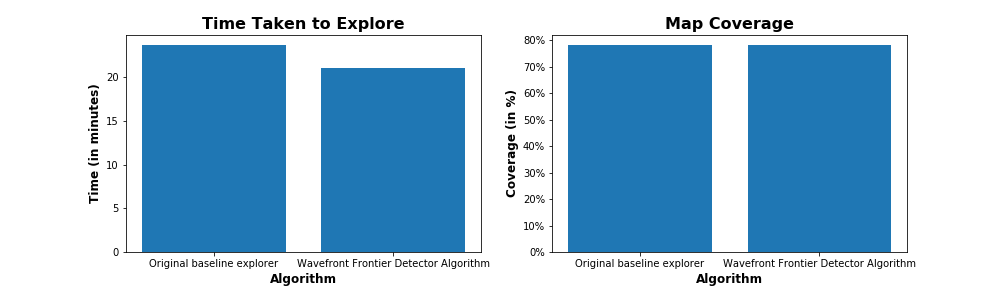
\includegraphics[scale=0.5]{images/Part2.png}
					\caption{Graphs showing how the exploration time and coverage differ for the reference(baseline) algorithm and our implementation of the explorer algorithm utilizing WFD.}
					\label{Part2}
				\end{figure}

	
	%%%%%%%%%%%%%%%%%%%%%%%%%%%%%%%%%%%%%%
	
	%%%%%%%%%%% PART 3 %%%%%%%%%%%%%%%%%
	\section{Mapping the Environment}
		The algorithm results obtained in the last chapter utilized a search grid that had knowledge of the real map when planning a route. However, in this example, the planner and the occupancy grid are both set to be unknown when the robot starts. This will test both the reactive planner and the frontier detection in conjunction. Whereas previously, the planner could decide if a destination is reachable, now the reactive planner will be used to handle this. As previously discussed, the validation of the start cell is disabled to prevent early termination of the planner. The results of the exploration are presented below in Fig. \ref{Part3}. 

		\begin{figure}[H]
			\centering
			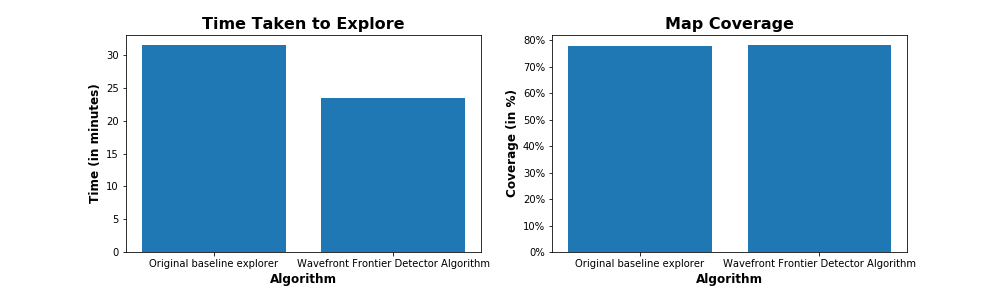
\includegraphics[scale=0.5]{images/Part3.png}
			\caption{Graphs showing how the exploration time and coverage differ for the reference(baseline) algorithm and our implementation of the explorer algorithm utilizing WFD in the case when the true search grid is not known to the planner.}
			\label{Part3}
		\end{figure}
	
	%%%%%%%%%%%%%%%%%%%%%%%%%%%%%%%%%%%%%%
	
	%%%%%%%%%%% PART 4 %%%%%%%%%%%%%%%%%
	\section{Information-Theoretic Path Planning}
		
		\subsection{Description of Entropy and Mutual Entropy}
			The information-Theoretic approach to path planning utilizes the concept of entropy. Entropy represents the uncertainty in the map. For a single cell the entropy would be given by the equation shown in Eq. \ref{eq:singleCellEntropy1}. In this equation $\textbf{c}$ represents a cell and $c$ represents the possible states of the cell. Therefore entropy is a sum over all of the possible states of the cell.

			\begin{equation}
				H \left(\textbf{c}\right) = - \sum_{c} p\left(\textbf{c}=c\right)\text{ln} \; p\left(\textbf{c}=c\right)
				\label{eq:singleCellEntropy1}
			\end{equation}
			
			In our example, cells are either known to be occupied/free or unknown. Additionally, the state of a cell can either be occupied or free. Therefore the above mentioned sum has only two terms. Furthermore given that the probability of a cell being occupied and the probability of a cell being free sum to 1, the sum depends on only one probability. This simplified version of the entropy of a cell can be found in Eq. \ref{eq:singleCellEntropy}. In this equation the probability $p\left(\textbf{c}\right)$ represents the probability of the cell being occupied. The occupancy grid for our simplified case consisting of cells with probabilities equal to 0, 0.5 or 1 can be shown to have cells of entropy as follows:

			\begin{align}
				\nonumber p\left(\textbf{c}\right) = 0 \; &: \; H \left(\textbf{c}\right) = -(1)\text{ln}(1)-\text{ln}(0) = 0 \\
				\nonumber p\left(\textbf{c}\right) = 0.5 \; &: \; H \left(\textbf{c}\right) = -(0.5)\text{ln}(0.5)-0.5\text{ln}(0.5) = \text{ln}2 \\
				\nonumber p\left(\textbf{c}\right) = 1 \; &: \; H \left(\textbf{c}\right) = -(0)\text{ln}(0)-1\text{ln}(1) = 0 \\
			\end{align}

			To compute the entropy of the whole map the expression in Eq. \ref{eq:mapEntropy1} needs to be evaluated. in this equation, $\textbf{M}$ represents possible map realizations (i.e. specific assignments of occupied/free to cells). The entropy is the sum over all possible map realizations.

			\begin{equation}
				H \left(\textbf{C}\right) = - \sum_{\textbf{M}} p\left(\textbf{M}\right) \text{ln} \; p\left(\textbf{M}\right)
				\label{eq:mapEntropy1}
			\end{equation}
			
			To compute $p(\textbf{M})$ we introduce the notation $p_\textbf{C}(\textbf{M})$ which signifies the probability that an occupancy grid $\textbf{C}$ can take a specific map realization $\textbf{M}$. Assuming independence between cells this can be expressed as shown in Eq. \ref{eq:mapProbability1}.
			
			\begin{equation}
				p_\textbf{C}(\textbf{M}) = \prod_{i} \prod_{j} p(c_{ij} = m_{ij})
				\label{eq:mapProbability1}
			\end{equation}
			
			This product can be broken down into two groups of cells: the group of known cells and the group of unknown cells. As this is mutually exclusive, there is no intersection between the two sets. We can therefore rewrite Eq. \ref{eq:mapProbability1} as a product of the known and unknown probabilities. The probability of the known portion can easily be computed, If the map realization $\textbf{M}_K$ is equal to the current known map realization $\textbf{M}_K^{known}$ then the probability is 1 otherwise the probability is 0. This can be described by a delta function which we shall label $\delta_{\textbf{C}_K}(\textbf{M}_K)$. Using these the following equations are formulated:

			\begin{equation}
				\begin{split}
					p_\textbf{C}(\textbf{M}) &= p_{\textbf{C}_K}(\textbf{M}_K) \cdot p_{\textbf{C}_U}(\textbf{M}_U) \\
					p_\textbf{C}(\textbf{M}) &= \delta_{\textbf{C}_K}(\textbf{M}_K) \cdot p_{\textbf{C}_U}(\textbf{M}_U) 
				\end{split}
				\label{eq:mapProbability2}
			\end{equation}

			By exploiting the nature of the delta function the map probability can be written as the following piecewise function:

			\[
				p_\textbf{C}(\textbf{M}) =
				\begin{cases}
					0 										& \text{if $\textbf{M}_K \neq \textbf{M}_K^{known}$} \\
					p_{\textbf{C}_U}(\textbf{M}_U) 			& \text{if $\textbf{M}_K = \textbf{M}_K^{known}$} 
				\end{cases}
			\]
			
			This piecewise function can be simplified further by considering the simple case studied in this coursework. In this example, cells are limited to 2 different states and if unknown they have the same probability of being occupied or free. Therefore the probability $p_{\textbf{C}_U}(\textbf{M}_U)$ can be rewritten as shown in Eq. \ref{eq:mapProbability3}. In this equation, $\mid \textbf{C}_U \mid$ represents the number of unknown cells. 

			\begin{equation}
				\begin{split}
					p_{\textbf{C}_U}(\textbf{M}_U) &= \prod_{i} p(c_{U,i} = m_{U,i}) \\
					&= \left(0.5\right)^{\mid \textbf{C}_U \mid}
				\end{split}
				\label{eq:mapProbability3}
			\end{equation}

			Now to compute the entropy of the map we consider Eq. \ref{eq:mapEntropy1}. Any map realizations where the known portion of the map doesn't match what is already know, will result in a probability of 0 and a 0 sum term. Therefore these map realizations can be ignored. The only map realizations that we need to consider are those where the known portion matches what is already known about the world. Given 2 possible states and $\mid \textbf{C}_U \mid$ unknown cells, there are $2^{\mid \textbf{C}_U \mid}$ different realizations of the unknown portion of the map. Additionally, due to the fact that in this simple case, the unknown cells have equal probability of being occupied and free, the probability of each of these realizations is equal.This results in Eq. \ref{eq:mapEntropy1} reducing to the form shown in Eq. \ref{eq:mapEntropy2}.

			\begin{equation}
				\begin{split}
					H \left(\textbf{C}\right) &= - \sum_{\textbf{M}} p\left(\textbf{M}\right)\text{ln} \; p\left(\textbf{M}\right) \\
					&= - 2^{\mid \textbf{C}_U \mid} \cdot \left(0.5\right)^{\mid \textbf{C}_U \mid} \text{ln} \left(0.5\right)^{\mid \textbf{C}_U \mid} \\
					&= - 2^{\mid \textbf{C}_U \mid} \cdot \left(2\right)^{-\mid \textbf{C}_U \mid} \text{ln} \left(0.5\right)^{\mid \textbf{C}_U \mid} \\
					&= - \mid \textbf{C}_U \mid \text{ln} \left(0.5\right) \\
					&= \mid \textbf{C}_U \mid \text{ln} \left(2\right)
				\end{split}
				\label{eq:mapEntropy2}
			\end{equation}

			It can be seen from this that the entropy in out case is directly proportional to the number of unknown cells. Now that we have a way of computing the current entropy of the map, we can utilize this in conjunction with another quantity to decide where the robot should travel to next. For this we introduce the mutual entropy. The mutual entropy is a measure of how much information is gained and it is this quantity that is to be maximized when choosing the next waypoint. To describe the mutual entropy, let us first assume that the robot travels to a point $\textbf{x}$ and observes the cells $\textbf{z}$. The new entropy of the map can be written as $H\left(\textbf{C}\mid\textbf{x},\textbf{z}\right)$. As we don't know the actual map, the observation $\textbf{z}$ that the robot makes is unknown to us. Therefore, we utilize the probability distribution of the unknown cells to produce an expected realization of the cells that are covered by the robot's lasers. This can be computed by producing a probability weighted sum of the Map Entropy over all the possible map realizations(as shown in Eq. \ref{eq:expectedMapEntropy}). This will be used to estimate the entropy of the map once the robot has travelled to the point $\textbf{x}$. 

			\begin{equation}
				H(\textbf{C}\mid\textbf{x}) = \sum_{\textbf{C}} p_{\textbf{C}_k}(\textbf{M})H(\textbf{C}\mid\textbf{x},\textbf{z}(\textbf{M}))
				\label{eq:expectedMapEntropy}
			\end{equation}

			The mutual entropy is the information gained by travelling to a point $\textbf{x}$ and is given by the expression in Eq. \ref{eq:mutualEntropy}

			\begin{equation}
				I(\textbf{x}) = H \left(\textbf{C}\right) - H(\textbf{C}\mid\textbf{x})
				\label{eq:mutualEntropy}
			\end{equation}

			The optimal cell to travel to $\textbf{x}^{*}$ is then given by the following maximization problem:

			\begin{equation}
				\textbf{x}^{*} = \argmax_{\textbf{x}}I(\textbf{x})
				\label{eq:optimalCell}
			\end{equation}

		\subsection{Evolution of Entropy over Time}

			\begin{figure}[H]
				\centering
				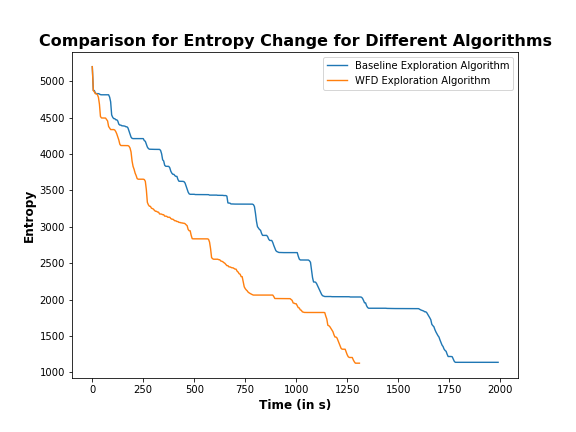
\includegraphics[scale=0.5]{images/EntropyChange.png}
				\caption{The evolution of entropy over time for two different exploration algorithms.}
				\label{EntropyChange}
			\end{figure}

			Using the equation for the entropy from Eq. \ref{eq:mapEntropy2}, the entropy of the map was computed at 5 second intervals. This was done for bot the baselines algorithm and our own implementation of the WFD algorithm. The results of this are shown in Fig. \ref{EntropyChange}. There are some distinct features in this plot. We can observe that both plots decrease as time evolves. This makes sense as when the explorer gains more knowledge about the environment, the uncertainty in the map decreases resulting in a lower entropy. In addition to this, a step like behaviour can be observed. This can be explained by the fact that the robot will not always be gaining new information. For example if a robot travels through a known region to get to a frontier, no new information will be gained for the time it travels through the known region. This results in no change in the map entropy. 
			\\
			\\
			We can also see that both explorers reach a similar final entropy. This is backed up by Fig. \ref{Part3} where both explorers have a similar final coverage. Due to the fact that entropy is proportional to the number of unknown cells, a similar coverage will result in a similar final map entropy. A notable difference between the two traces is that despite reaching the same final entropy value, our WFD implementation reached this value much quicker that the baseline algorithm. In addition to this, the gradient of the entropy plot is higher for our WFD implementation than the baseline algorithm. This suggests that our WFD implementation is able to gain information about the environment quicker than the baseline algorithm is. Therefore we are able to conclude with confidence that our WFD implementation is better than the baseline explorer algorithm. 
	%%%%%%%%%%%%%%%%%%%%%%%%%%%%%%%%%%%%%%
	
	\newpage
	\bibliographystyle{IEEEtran}
	\bibliography{references}
	\newpage
	\appendix
	\appendixpage
	\addappheadtotoc
	
\end{document}